\section{Results}
In this section, we first compare the number of GMRES iteration needed by 
ANMG-DSA and ANMG-P1SA to solve a test case. Then, both the number of GMRES 
iterations and the elapsed time are compared for three methods :
\begin{itemize}
\item Sweep preconditioning (S).
\item DSA with optimal transport correction preconditioning (DSA).
\item Angular multigrid with DSA preconditioning (ANMG-DSA).
\end{itemize}
The tests use a homogeneous medium and Fokker-Planck cross
sections with $\alpha=1$. $\Sigma_{t}$ is chosen to be equal to
$\Sigma_{s,0}$. The quadrature is the Gauss-Legendre-Chebyshev Galerkin
quadrature. The domain is a $5cm$ side square and the uniform mesh is composed
of 50 by 50 
cells. The GMRES solver is converged to a relative tolerance of $10^{-4}$. To
conclude this section, the eigenvalue spectrum of the three methods is
compared on a example.
\subsection{Comparison between ANMG-DSA and ANMG-P1SA}
The number of GMRES iterations needed to solve ANMG-DSA and
ANMG-P1SA are compared. It should be noticed that it is
harder to solve the P1SA, which positive definite, than the DSA which is
symmetric positive definite. The comparison is done for $S_4$, $S_8$ and
$S_{16}$. 
\begin{table}[H]
\begin{center}
\begin{tabular}{|c|c|c|c|c|c|}
\hline
\multicolumn{2}{|c|}{$S_4$} & \multicolumn{2}{c|}{$S_8$} &
\multicolumn{2}{c|}{$S_{16}$}\\
\hline
ANMG-DSA & ANMG-P1SA & ANMG-DSA & ANMG-P1SA & ANMG-DSA & ANMG-P1SA\\
\hline
17 &  15 & 23 & 28 & 42 & 70\\
\hline
\end{tabular}
\caption{Number of GMRES iterations}
\end{center}
\end{table}
From this result, it can be seen than ANMG-DSA outperforms ANMG-P1SA except for
$S_4$. When the anisotropy of the problem increases, the advantage of ANMG-DSA
over ANMG-P1SA increases. For this reason, only the ANMG-DSA will be compared
to Sweep and DSA preconditioning in the next two tests.
\subsection{Volumetric source}
For this test, there is an uniform isotropic source of intensity 10 $n/(cm^3s)$. 
We compare the results for the following quadrature order : $S_4$, $S_8$ and 
$S_{16}$. The thickness of the slab varies from
50 to 680 mean-free-path but stays constant at five transport mean-free-path.
\begin{table}[H]
\begin{center}
\begin{tabular}{|c|c|c|c|c|c|c|c|c|}
\hline
\multicolumn{3}{|c|}{$S_4$} & \multicolumn{3}{c|}{$S_8$} & 
\multicolumn{3}{c|}{$S_{16}$} \\
\hline  
S & DSA & ANMG-DSA & S & DSA & ANMG-DSA & S & DSA & ANMG-DSA\\
\hline
63 & 28 & 17 & 251 & 67 & 23 & 10840 & 175 & 42 \\
\hline
\end{tabular}
\caption{Number of GMRES iterations}
\end{center}
\end{table}
\begin{table}[H]
\begin{center}
\begin{tabular}{|c|c|c|c|c|c|c|c|c|}
\hline
\multicolumn{3}{|c|}{$S_4$} & \multicolumn{3}{c|}{$S_8$} & 
\multicolumn{3}{c|}{$S_{16}$} \\
\hline  
S & DSA & ANMG-DSA & S & DSA & ANMG-DSA & S & DSA & ANMG-DSA\\
\hline
283 & 1067 & 667 & 4351 & 4147 & 1331 & 67948 & 17595 & 5226 \\
\hline
\end{tabular}
\caption{Elapsed time (s)}
\end{center}
\end{table}
It can be noticed that while ANMG-DSA needs the least iterations to converge, it is
not always the fastest method. This is due to the work required by the extra
sweeps. However, as the anisotropy of the problem increases the advantage of
ANMG-DSA becomes obvious. For the $S_{16}$ quadrature, ANMG-DSA requires 20 times 
less iterations and 12 times less time than the sweep preconditioning. 
Compared to DSA, ANMG-DSA needs four times fewer iterations and three times less 
time. It is interesting to note that DSA is never more efficient (elapsed
time and number of iterations) than ANMG-DSA.

\subsection{Beam problem}
Now, we compare the number of GMRES iterations and the time needed to solve a
beam problem. We use a $S_8$ quadrature and there is an incoming flux coming
from the left for $y\in [2cm,3cm]$ of intensity 10 $n/(cm^3s)$. The flux is
coming from the most normal directions of the quadrature.
\begin{table}[H]
\begin{center}
\begin{tabular}{|c|c|c|}
\hline
235 & 60 & 26 \\
\hline
\end{tabular}
\caption{GMRES iterations}
\end{center}
\end{table}

\begin{table}[H]
\begin{center}
\begin{tabular}{|c|c|c|}
\hline
3855 & 2287 & 1227\\
\hline
\end{tabular}
\caption{Elapsed time (s)}
\end{center}
\end{table}
These results confirm the previous ones and show the advantage of the angular
multigrid preconditioning over the DSA preconditioning.

%In this problem, there is an incoming flux of intensity 10 $n/(cm^3s)$ 
%coming from the left. The flux is coming from the most normal directions
%of the $S_{16}$ quadrature. 
%\begin{table}[H]
%\begin{center}
%\begin{tabular}{|c|c|c|}
%\hline  
%S & DSA & ANMG-DSA \\
%\hline
%768 & 169 & 43 \\
%\hline
%\end{tabular}
%\caption{GMRES iterations}
%\end{center}
%\end{table}
%\begin{table}[H]
%\begin{center}
%\begin{tabular}{|c|c|c|}
%\hline  
%S & DSA & ANMG-DSA \\
%\hline
%48009 & 14995 & 4623\\
%\hline
%\end{tabular}
%\caption{Elapsed time (s)}
%\end{center}
%\end{table}
%These results are very similar to the previous ones and confirm the advantages
%of ANMG-DSA over DSA and sweep preconditioning. 

\subsection{Spectrum}
Now, the eigenvalue spectrum is compared on an example. The set-up of the
problem is similar to the previous one. We use a $S_8$ quadrature and the
domain is discretized using 5 by 5 cells.

\begin{figure}[H]
\centering
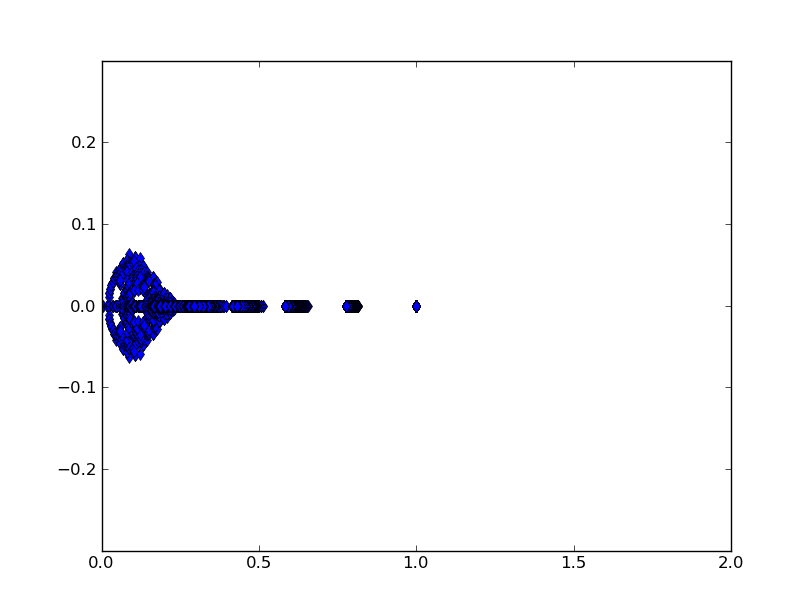
\includegraphics[width=9cm]{s8_5_5}
\caption{Spectrum of the Sweep preconditioned system}
\end{figure}
% 1.0000
% 0.0048255

% S16 : condition number : 40

\begin{figure}[H]
\centering
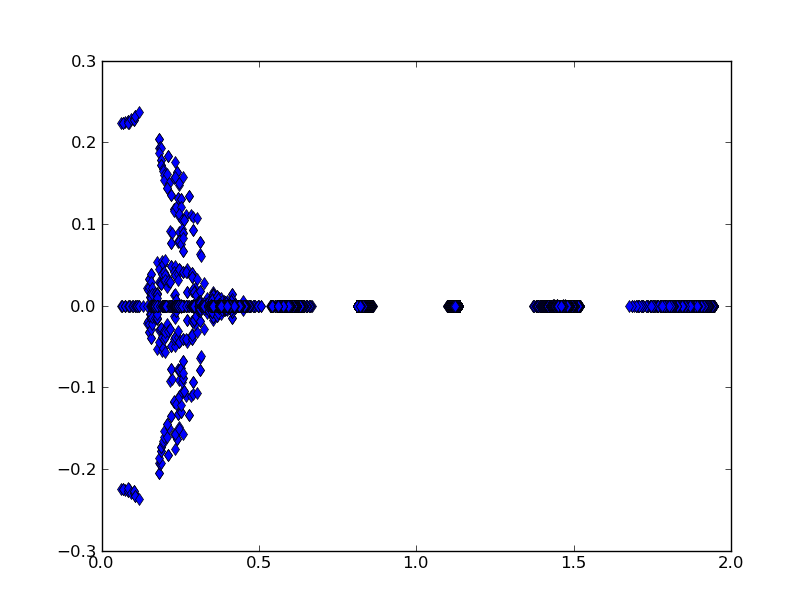
\includegraphics[width=9cm]{d_s8_5_5}
\caption{Spectrum of the DSA preconditioned system}
\end{figure}
% 1.94563117
% 0.0621324 \pm 0.224359i

% S16 : condition number : 158.9499131
% 1.98537
% 0.017012876394 \pm 0.11949429816i

\begin{figure}[H]
\centering
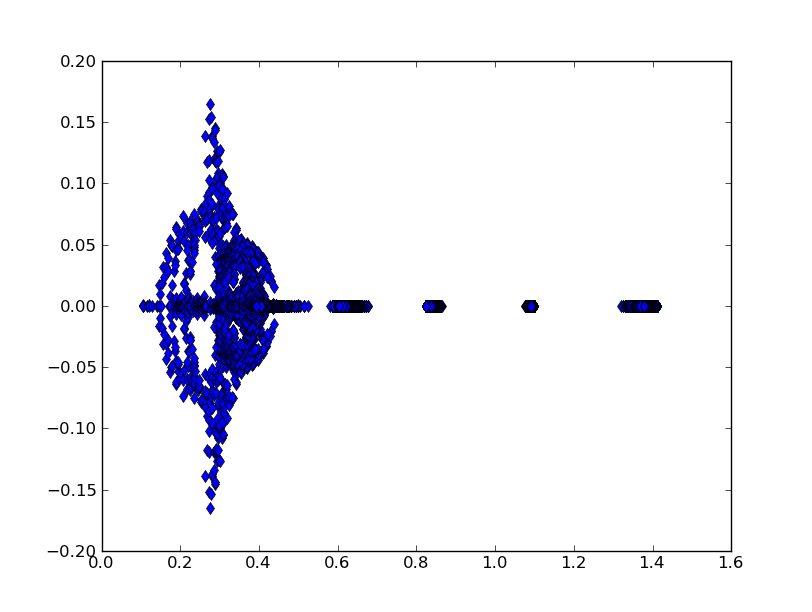
\includegraphics[width=9cm]{p_s8_5_5}
\caption{Spectrum of the Angular Multigrid with DSA preconditioned system}
\end{figure}
% 1.41172
% 0.1051087

On these figures, we can see that the DSA moves the eigenvalues away from
zero. This explains the faster convergence of GMRES with DSA preconditioning
compared to Sweep preconditioning. ANMG moves the
eigenvalues even further away than DSA and gathers them compared to DSA.
It is obvious from these figures that ANMG should converge much faster than
DSA which is what was observed in the previous tests. 
